\documentclass[a4paper,11pt]{article}

\usepackage{fullpage}
\usepackage{color}
\usepackage{hyperref}
\usepackage{amsmath}
\usepackage{amssymb}
\usepackage{tikz}
\usepackage{tabularx}
\usepackage{booktabs}
\usepackage{amsmath}
\usepackage{multirow}
\usepackage{layouts}
\usepackage{array}
\usepackage{pgf}
\usepackage{tikz}

\usepackage{amssymb}
\usepackage{graphics}
\usepackage{fancyhdr}
\usepackage{eucal}
\usepackage{ifthen}
\usepackage{ifpdf}
\usepackage{lmodern}
\usepackage{amsthm}
\usepackage{catoptions} % For \Autoref


\usetikzlibrary{positioning}

\hypersetup{
  colorlinks,%
    citecolor=black,%
    filecolor=black,%
    linkcolor=black,%
    urlcolor=mygreylink     % can put red here to visualize the links
}

\definecolor{hlcolor}{rgb}{1, 0, 0}
\definecolor{mygrey}{gray}{.85}
\definecolor{mygreylink}{gray}{.30}
\textheight=8.6in
\raggedbottom
\addtolength{\oddsidemargin}{-0.375in}
\addtolength{\evensidemargin}{0.375in}
\addtolength{\textwidth}{0.5in}
\addtolength{\topmargin}{-.375in}
\addtolength{\textheight}{0.75in}


\newcommand{\resheading}[1]{{\large \colorbox{mygrey}{\begin{minipage}{\textwidth}{\textbf{#1 \vphantom{p\^{E}}}}\end{minipage}}}}

\newcommand{\mywebheader}{
  \begin{tabular}{@{}p{5in}p{4in}}
  {\resheading{Assignment 2: Single Agent Learning}} & {\Large 5 October, 2012}\\\vspace{0.2cm}
  \end{tabular}}

\begin{document}


\begin{center}
{\LARGE \textbf{Autonomous Agents}}\\ [1em]
\end{center}
\mywebheader

\begin{center}
{\Large By:} \\ \vspace{0.1cm}
{\Large Paris Mavromoustakos} \\  \vspace{0.1cm}
{\Large Georgios Methenitis} \\ \vspace{0.1cm}
{\Large Patrick de Kok} \\ \vspace{0.1cm}
{\Large Marios Tzakris}
\end{center}




\section*{Introduction}

In this assignment, we implement the learning scenario: the transition function is unknown to the agents, and so is the reward structure. We introduce model-based algorithms, which give agents the ability to learn high-reward policies while ignoring the model.  \\
Our code is based on the previous assignment, on which we added the classes necsessary to implement learning algorithms. Moreover, we have explicitly used the 21 statespace environment representation which reduced our algorithms' runtime on the previous assignment.


\section*{Exercise 1}

In this first exercise, we have implemented the Q-Learning algorithm with $\epsilon$-greedy action selection, as described  in chapter 6.5 of the Sutton and Barto book.\\
On each step of this algorithm, we chose an action $a$ of state $s$, and observed the next state and reward we got from it. Then, we updated the Q-learning table according to the following update rule: \\ 

$Q(s,a) \leftarrow  Q(s,a) + \alpha \left[ r + \gamma  max_{a'} Q(s',a') - Q(s,a)\right]$ \\

In this update rule, $Q(s,a)$ represents the value of the Q-learning table based on the previous step, while $Q(s',a')$ represents the observed state and possible actions, after action a is chosen. $Q(s,a)$ could be written as $Q(s_t,a_t)$ and $Q(s',a')$ as $Q(s_{t+1}, a_{t+1})$.\\
$\alpha$ represents the algorithm's learning rate, whereas $\alpha =0$ means that the Q-learning table will not be updated (the agent is not learning anything at all), while $\alpha =1$ means that that the agent learns based only on its immediate past.\\
$\gamma$ represents the discount factor, in the same way as described in DP algorithms, and $max_{a'}$ represents the action which is most likely to return the maximum reward among all the possible actions in state $s'$.

$\epsilon$ was given the value of 0.1 and the Q-learning table was initialized with 15.0 being assigned to all values. 


The figures below indicate the performance of the predator over time, given different values for $\alpha$ , and different values for $\gamma$.




\begin{center}
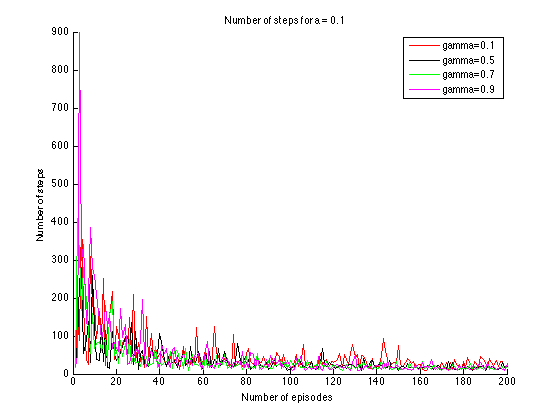
\includegraphics[width=1.0\textwidth,height=0.4\textheight]{a1.png}
\label{Figure 1}
Figure 1. 	Comparing implementations for different discount factors with $\alpha = 0.1$\vspace{1cm}
\end{center}

\begin{center}
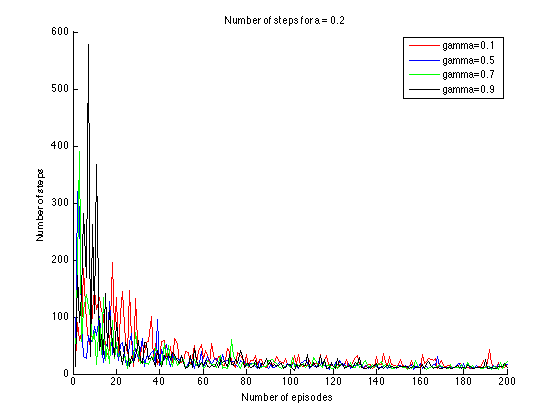
\includegraphics[width=1.0\textwidth,height=0.4\textheight]{a2.png}
\label{Figure 2}
Figure 2. 	Comparing implementations for different discount factors with $\alpha = 0.2$\vspace{1cm}
\end{center}

\begin{center}
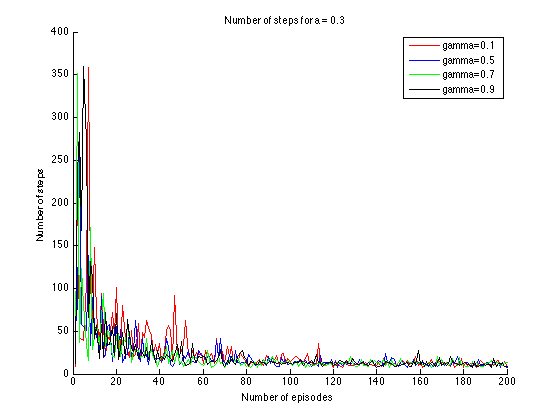
\includegraphics[width=1.0\textwidth,height=0.4\textheight]{a3.png}
\label{Figure 3}
Figure 3. 	Comparing implementations for different discount factors with $\alpha = 0.3$\vspace{1cm}
\centering
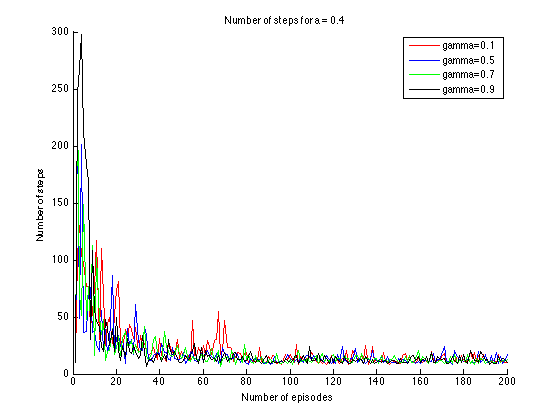
\includegraphics[width=1.0\textwidth,height=0.4\textheight]{a4.png}
\label{Figure 4}
Figure 4. 	Comparing implementations for different discount factors with $\alpha = 0.4$\vspace{1cm}
\end{center}

\begin{center}
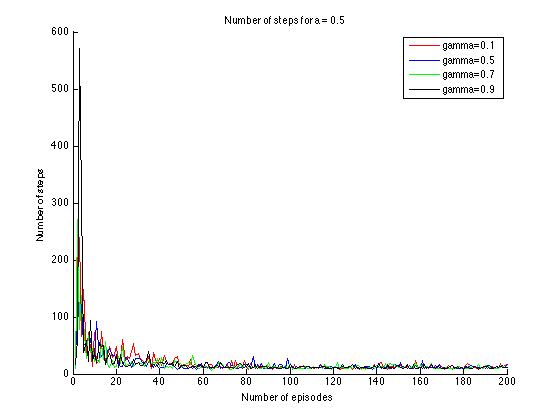
\includegraphics[width=1.0\textwidth,height=0.4\textheight]{a5.png}
\label{Figure 5}
Figure 5. 	Comparing implementations for different discount factors with $\alpha = 0.5$\vspace{1cm}
\end{center}
Figures 1-5 clearly indicate how the predator learns faster while we increment the value of $\alpha$. Figure 1 shows us that for $\alpha = 0.1$ the predator needs about 150 episodes to converge to the optimal policy. However, while we increase alpha, the predator will need less episodes for its Q-learning table to converge. \\
Increasing the value of $\alpha$ means that we consider the most recent information we observe, more important. A value of $\alpha = 0$ would mean that the predator is not learning at all, while $\alpha = 1$ means that the predator only obtains information from its immediately previous actions. 
 
\section*{Exercise 2}

In this exercise we have implemented Q-learning with $\epsilon$ -greedy action decision for different values for $\epsilon$ , using different initial values for the Q-learning table each time. We have used 3 different values for the initialization of the Q-table, a pessimistic one (5), a realistic one (10) and an optimistic one (15), to see how the agent behaves for different values of $\epsilon$ in each case. On the pessimistic implementation, we expect the agent to converge to the optimal path really fast (given low values for $\epsilon$). On the other hand, the optimistic implementation will cause more of an exlporatory behavior.


In figure 6 we are testing $\epsilon$ -greedy action selection for the optimistic, realistic and pessimistic initialization of the Q-learning table. As shown, the pessimistic value helps the agent converge to the optimal path faster than the other implementations (this happens in this case, where we only have one absorbing state), while the optimistic value lets the agent explore a lot more before it converges.


\begin{center}

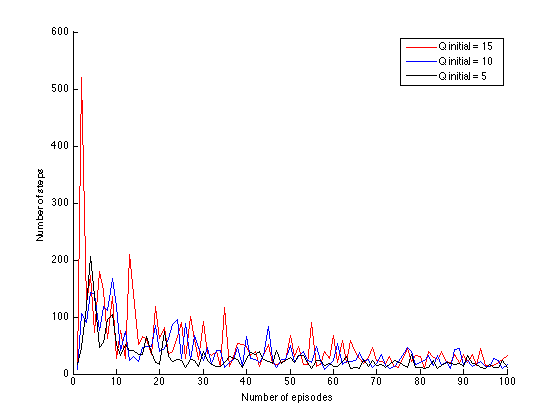
\includegraphics[width=1.0\textwidth,height=0.4\textheight]{realpesopt.png}
\label{Figure 5}
Figure 6. 	Comparing implementations for different values for $Q_{initial}$  with $\alpha = 0.1$ , $\gamma=0.7$ 

($\epsilon$ -greedy action selection).\vspace{1cm}

\end{center}


We have chosen particular values for $\epsilon$ to test how, and what the predator will learn to do. For $\epsilon = 0$, the predator will always choose the action for which the Q-learning table has maximum value, thus, the agent will converge to the optimal path really fast if the initial values of the Q-table are lower than the immediate reward of the absorbing state, but it will become explorative if the Q-table values are optimistically initialized.


If $\epsilon = 0.1$, the agent will try to exploit the action for which the Q-table has the maximum value with a probability of $1-\epsilon = 0.9$. That means that our predator is trying to exploit more than it is trying to explore, and there is a small probability that it will not choose the action it considers optimal.

We have used the value of 0.8 for $\epsilon$ aswell, because in this case, each possible action for the predator might have the same probability to be chosen. For example, if the predator has 5 possible actions, there will be $1-\epsilon = 0.2$ probability for the "optimal" action to be chosen, and each of the other possible states will also have $\epsilon /4 = 0.2$ probability to be chosen. As a consequence, in the best case scenario our agent will be moving randomly. If there are less than 5 possible moves, he will be most likely be choosing one of the "non-optimal" moves.

Finally, we have also included $\epsilon = 0.99$ in our experimentation, for the reason that this value leaves almost zero probability for the agent to choose the optimal action. So, what happens in this case is that the predator learns not to use the optimal action each time he has to take a decision, so as we see in the graphs, the number of steps it takes him to find the prey is increased dramatically as time goes by.

\begin{center}

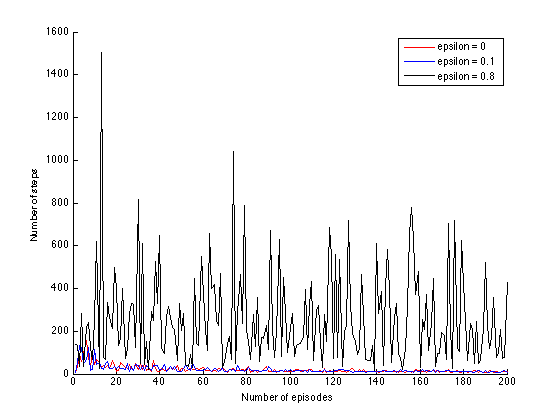
\includegraphics[width=1.0\textwidth,height=0.4\textheight]{epsilonvalues.png}
\label{Figure 1}
Figure 7. Comparing different values of $\epsilon$ with $\epsilon$ -greedy action selection. For $\epsilon = 0.8$ the agent will be deciding its actions almost randomly. \vspace{1cm}
\end{center}


\begin{center}

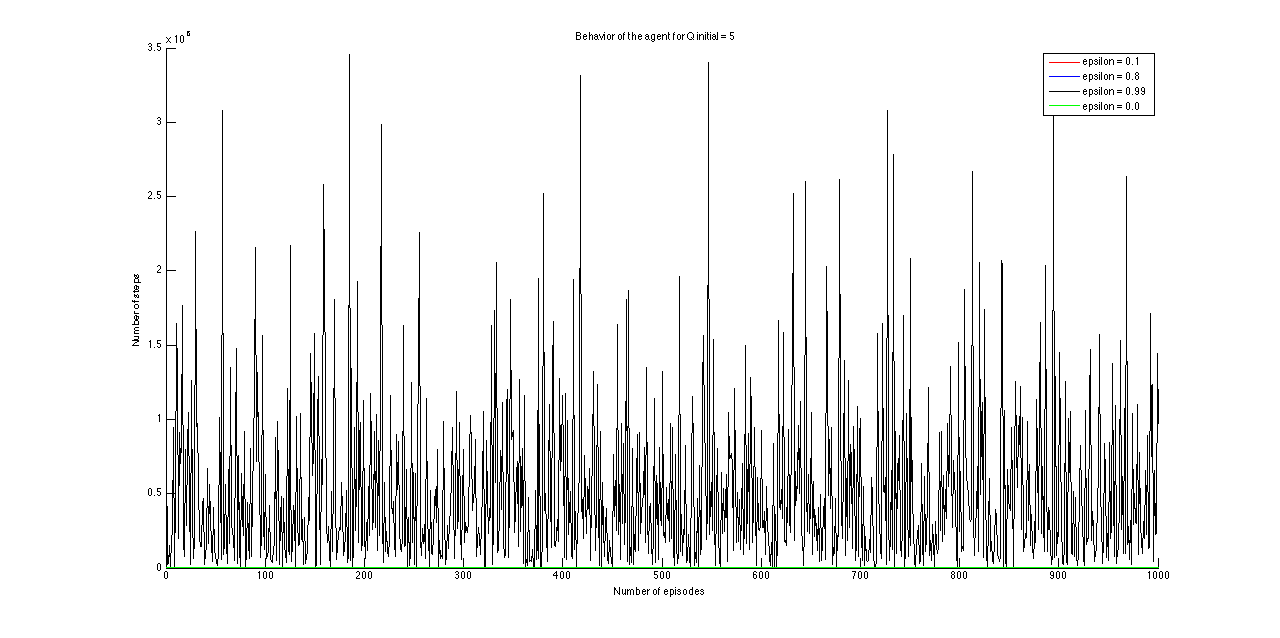
\includegraphics[width=1.0\textwidth,height=0.4\textheight]{epsilonsQ5.png}
\label{Figure 1}
Figure 8. When the value of $\epsilon$ is close to 1, the agent tends to avoid the maximum expected reward states. \vspace{1cm}
\end{center}

\newpage
It should be pointed out that for $Q_{initial} = 10$ and $Q_{initial} = 15$ the graphs are quite similar, with the plot of $\epsilon = 0.99$ dominating the other values. We only included this graph to show how this particular value of $\epsilon$ affects the behavior of the agent.
\section*{Exercise 3}

In this exercise we implemented softmax action selection instead of $\epsilon$ -greedy. 
Softmax differs from $\epsilon$ -greedy in one important detail: $\epsilon$ -greedy divides probability equal to $\epsilon$ among all the "non-optimal" possible actions, while softmax distributes weighted probability analogically to the actions' values. This means, that in $\epsilon$ -greedy the worst possible action has the same probability to be chosen as the second-to-best action, while in softmax, the worst possible action will always have the lowest probability to be chosen.

Softmax chooses each action with probability equal to $\frac{\varepsilon ^{Q_t(a)/ \tau}}{\sum^n_{b=1}\varepsilon ^{Q_t(b)/ \tau}}$
where $\tau$ is a positive variable called "temperature". If $\tau >> 0$ the possible actions tend to be equiprobable, however, if $\tau \rightarrow 0$ softmax tends to choose the next action greedily.

In our simulation, we found out that $\epsilon$ -greedy and softmax action selection are very much alike, and do not show any important difference. In figure 9, we have plotted the behavior of the agent with $\epsilon$ -greedy and softmax implementation.

\begin{center}
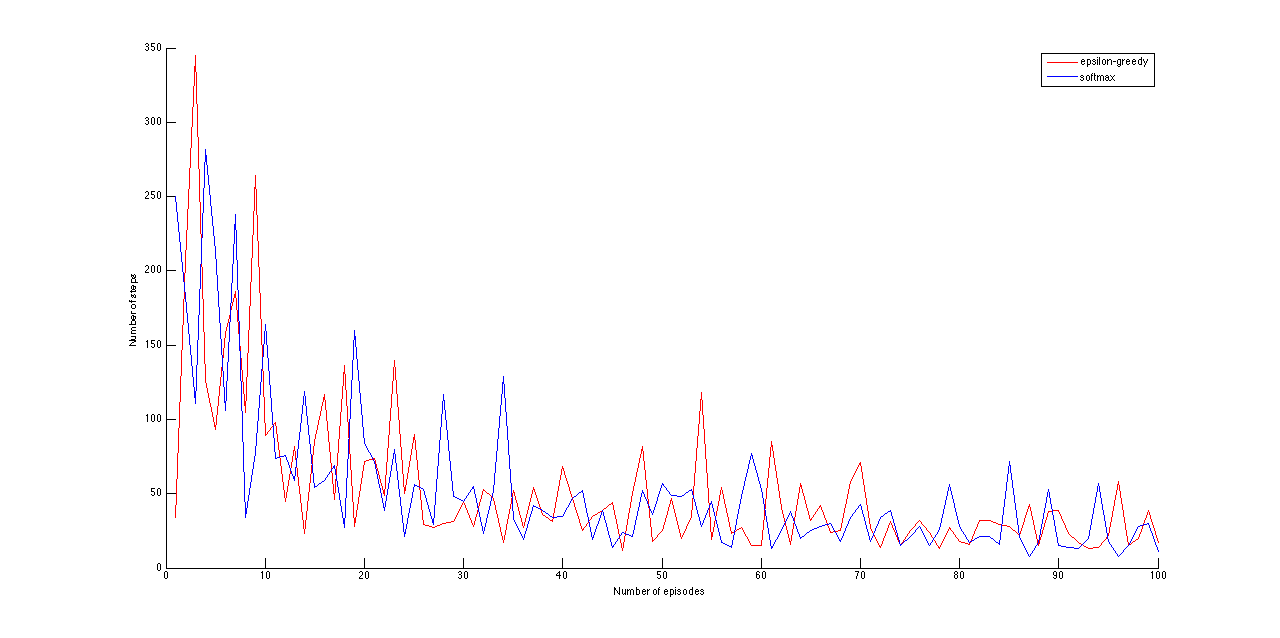
\includegraphics[width=1.0\textwidth,height=0.4\textheight]{s1e1.png}
\label{Figure 1}
Figure 9. Comparing $\epsilon$ -greedy and softmax implementations in Q-learning for $\alpha = 0.1$ , $\gamma = 0.7$, $\tau = 0.1$, $\epsilon = 0.1$ and $Q_{initial} = 15$.
\end{center}
\section*{Exercise 4}
In the last exercise we went past the Q-learning algorithm and implemented the Sarsa, On-policy Monte Carlo and Off-policy Monte Carlo algorithms. 	
\subsection*{Sarsa}
Sarsa is an on-policy temporal difference control method. On-policy TD methods use a certain policy ($\epsilon$ -greedy, softmax), which defines their future actions, and based on the reward they receive, they evaluate this policy.

On the other hand, off-policy TD methods do not "stick" to one particular policy, but can learn different policies and use the one for which they receive the best results. Another difference between on-policy and off-policy TD methods is that the latter update their value functions based on hypothetical actions, which actually they do not take, while on-policy TD methods are strictly based on the experience they gain from performing those actions.

Sarsa and Q-learning have a lot in common, but there is an important difference that discriminates the two algorithms: When agent is at state $s$ and takes action $a$, Q-learning will update the Q table based on this action's reward. However, Sarsa will further observe the next state-action pair $(s',a')$ that derives from the next state $s'$ produced by action $a$. So, obviously, Sarsa needs two action selection steps, while Q-learning only needs one. Thus, Sarsa is considered an on-policy TD control method while Q-learning is considered to be off-policy.

On figure 10 we can look at a comparison between Q-learning and Sarsa algorithms' behavior. According to the graph, the two algorithms have quite similar results.

\begin{center}
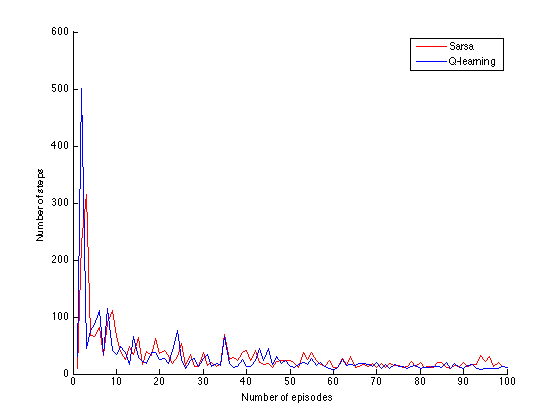
\includegraphics[width=1.0\textwidth,height=0.4\textheight]{sarsaQ.png}
\label{Figure 1}
Figure 10. Comparing Sarsa and Q-learning algorithms for $\alpha = 0.3$, $\gamma = 0.7$ and $\epsilon = 0.2$.
\end{center}

\subsection*{On-policy Monte Carlo}


\subsection*{Off-policy Monte Carlo}
\begin{center}
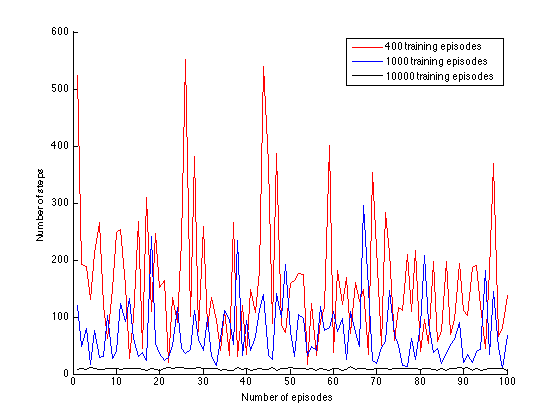
\includegraphics[width=1.0\textwidth,height=0.4\textheight]{offpolicyMC.png}
\label{Figure 1}
Figure 11. Comparing Off-Policy Monte Carlo for different numbers of training episodes, with $\epsilon$ -greedy action selection ($\alpha = 0.2$, $\gamma = 0.7$).
\end{center}

\begin{center}
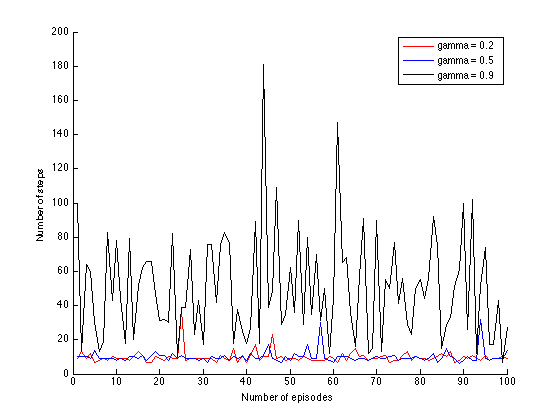
\includegraphics[width=1.0\textwidth,height=0.4\textheight]{offpolicygamma.png}
\label{Figure 1}
Figure 11. Comparing Off-Policy Monte Carlo for different values of $\gamma$, for 10000 training episodes.
\end{center}

\section*{Conclusion}

\end{document}

